\subsection{External clip evaluation and diagnostic analyses}

All 1,440 external clips and 11,520 sampled frames meet the frozen eligibility rules, giving 100\% maximum achievable coverage without model-outcome filtering. Table~\ref{tab:external} summarizes disagreement for both backbones, checkpoint states and annotation references. Changing the reference from raw responses to calm/neutral-merged responses scores the same predictions and accepted clips; it does not change inference or selection.

\begin{table}[t]
\caption{External disagreement at 80\% MSP coverage (\%): means of three seed-specific risks, not an ensemble. Every model accepts its own 1,152 of 1,440 clips}\label{tab:external}
\centering\small\begin{tabular}{lllrrr}\toprule
Backbone & State & Reference & Soft & Uniform & Tie-Uniform\\\midrule
Swin-T & Selected & Raw & 68.37 & 67.75 & 67.42\\
Swin-T & Selected & Merged & 60.72 & 60.62 & 60.03\\
Swin-T & Epoch 12 & Raw & 68.25 & 68.03 & 67.45\\
Swin-T & Epoch 12 & Merged & 60.47 & 61.37 & 60.16\\
ResNet-18 & Selected & Raw & 71.49 & 69.66 & 70.73\\
ResNet-18 & Selected & Merged & 63.20 & 61.88 & 62.46\\
ResNet-18 & Epoch 12 & Raw & 71.32 & 69.62 & 70.47\\
ResNet-18 & Epoch 12 & Merged & 63.24 & 61.96 & 62.35\\
\bottomrule\end{tabular}\par\smallskip
Raw retains nine human responses; Merged adds calm to neutral and retains none. Neither is intended-expression accuracy. The model predictions and accepted IDs are unchanged between references.\par
\end{table}

\begin{table}[t]
\caption{Principal external comparison: validation-selected Swin-T Soft minus Uniform at 80\% MSP coverage (percentage points). Negative favors Soft}\label{tab:externalseeds}
\centering\small\begin{tabular}{lrrrrl}\toprule
Reference & Seed 17 & Seed 42 & Seed 89 & Mean & Actor interval\\\midrule
Raw & -0.052 & +2.639 & -0.755 & +0.611 & [+0.23, +1.09]\\
Merged & -1.276 & +2.483 & -0.903 & +0.101 & [-0.26, +0.59]\\
\bottomrule\end{tabular}\par\smallskip
Percentile 95\% actor-cluster intervals use shared actor multiplicities and reranking within 5,000 replicates, conditional on these three fitted pairs and observed votes. They do not quantify seed-population, new-rater or unrestricted demographic uncertainty.\par
\end{table}

The principal external contrast does not reproduce the source-dataset advantage consistently across seeds (Table~\ref{tab:externalseeds}). Under the raw reference, the +0.611 pp mean is driven by the larger positive contrast for seed 42, which outweighs the negative contrasts for seeds 17 and 89. Its actor-cluster interval lies above zero, but describes actor-sampling sensitivity conditional on these fitted pairs and observed votes. Under the merged reference, the interval crosses zero. Neither result establishes equivalence or a stable external ordering across retraining.

Checkpoint state and annotation reference further qualify the comparison. Under the merged reference, all three epoch-12 Swin-T contrasts favor Soft, whereas the validation-selected contrasts have mixed directions. The complete per-seed results remain in the supplement. The external evaluation therefore tests the transfer of the frozen pipelines as a whole; it does not isolate supervision from differences in capture conditions, population or frame aggregation.

\begin{figure}[tp]\centering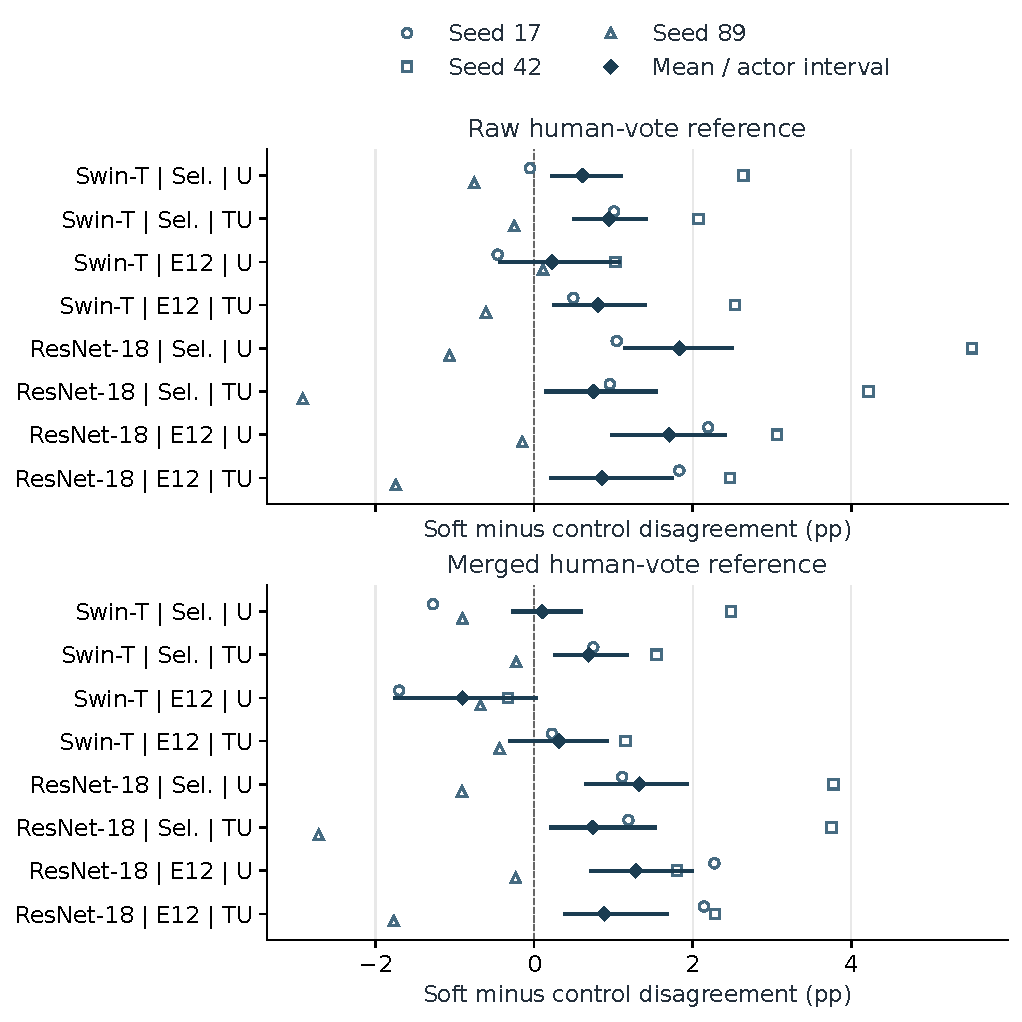
\includegraphics[width=\linewidth]{submission_reader_2026_10_13/source/figures/ExternalContrasts.pdf}

\caption{External disagreement differences at 80\% MSP coverage, using separate model rankings. Hollow symbols show all three paired seed contrasts; the diamond and bar show their mean and conditional 95\% actor-cluster interval. Vertical offsets separate the seeds. Sel.: selected checkpoint; E12: fixed-epoch checkpoint; U: Uniform; TU: Tie-Uniform. Both panels share the horizontal scale; negative favors Soft. Intervals describe actor-sampling sensitivity for these fitted pairs and votes, not uncertainty over new seeds, raters or populations. Zero denotes equal mean disagreement, not equivalent predictions or accepted sets}\label{fig:external}\end{figure}

\begin{table}[htbp]
\caption{Principal external risk accounting: validation-selected Swin-T, means across three seeds (\%). Components use the same population as total risk}\label{tab:externalaccounting}
\centering\small\begin{tabular}{lllrrrr}\toprule
Population & Supervision & Ref. & Risk & Unsup. & Ambig. & Excess\\\midrule
All eligible & Soft & Raw & 71.06 & 11.90 & 16.81 & 42.36\\
All eligible & Uniform & Raw & 70.81 & 11.90 & 16.81 & 42.11\\
All eligible & Soft & Merged & 64.84 & 3.14 & 20.23 & 41.47\\
All eligible & Uniform & Merged & 64.81 & 3.14 & 20.23 & 41.44\\
80\% MSP & Soft & Raw & 68.37 & 14.00 & 16.61 & 37.76\\
80\% MSP & Uniform & Raw & 67.75 & 13.58 & 16.59 & 37.58\\
80\% MSP & Soft & Merged & 60.72 & 3.31 & 20.78 & 36.64\\
80\% MSP & Uniform & Merged & 60.62 & 3.30 & 20.57 & 36.75\\
\bottomrule\end{tabular}\par\smallskip
All eligible: 1,440 clips per state. 80\% MSP: 1,152 independently ranked clips per state. Unsup. is unsupported vote mass; Ambig. is supported ambiguity. All-eligible components are not substituted for accepted-set components. Rounding can prevent displayed components from summing exactly.\par
\end{table}

The risk accounting identifies excess disagreement as the largest component both across all eligible clips and at 80\% MSP coverage (Table~\ref{tab:externalaccounting}). For validation-selected Swin-T Soft under the raw reference, the all-eligible excess is 42.36 percentage points, compared with 11.90 points of unsupported vote mass. Missing output categories alone therefore do not explain the poor transfer. The decomposition describes disagreement rather than its cause, and accepted-set components must be read on their own population rather than substituted from all-eligible averages.

The post hoc diagnostics show that neutral dominates accepted predictions in all three validation-selected Swin-T seeds: 67.0--70.0\% for Soft and 62.7--68.3\% for Uniform. The supplementary vote-weighted matrices and temporal summaries retain all six principal matrices and all eight temporal bins. Neutral probability is highest in the first bin and falls toward the middle, while frame-to-clip argmax agreement also varies across bins. These patterns describe the frozen outputs; they do not establish a cause of transfer failure or measure frame accuracy, since the human judgments apply to whole clips.

Online Resource 8 retains all 36 external states, category frequencies, raw-reference vote mass, raw/merged matrices and temporal summaries. The supplementary score/coverage and fixed-image comparisons provide the complete sensitivity results without changing the primary external comparison.
